% !TeX spellcheck = fr_CA
\documentclass[letterpaper, 12pt]{article}

% Encoding
\usepackage[utf8]{inputenc}
\usepackage[T1]{fontenc}

% Margins
\usepackage[top=2.5cm, bottom=2.5cm, left=2.5cm, right=2.5cm]{geometry}
% One half spacing
\usepackage{setspace}
\onehalfspacing
% Paragraph indentation
\setlength{\parindent}{0cm}
% Page numbering to the right
\usepackage{fancyhdr}
\pagestyle{fancy}
\fancypagestyle{plain}{\pagestyle{fancy}}
\fancyhf{} % clear all header and footer fields
\fancyfoot[R]{\thepage}
\renewcommand{\headrulewidth}{0cm}
\renewcommand{\footrulewidth}{0cm}
% Footnotes
\usepackage[bottom]{footmisc}

% Abstract
\usepackage{abstract}
% Table of contents, list of figures and tables
\usepackage{tocloft}
\usepackage[notindex, nottoc, notlof, notlot]{tocbibind}
% List of abbreviations
\usepackage{nomencl}
\makenomenclature
% Appendices
\usepackage[title, titletoc]{appendix}
% Bibliography
\usepackage[numbers]{natbib}
\usepackage{url}
\def\UrlBreaks{\do\/\do-}

% Figures
\usepackage{float, graphicx}
% Tables
\usepackage{booktabs, longtable, fonttable}
% SI units
\usepackage[squaren, Gray]{SIunits}
% Mathematics
\usepackage{amsmath, amssymb, mathrsfs}
% Drawings
\usepackage{tikz}
% Hypertext
\usepackage[colorlinks=false, pdfborder={0 0 0}]{hyperref}

% Document in french
\usepackage[french]{babel}

\usepackage{listings}
\usepackage{pdflscape}

% Matrice augmenté
\makeatletter
\renewcommand*\env@matrix[1][*\c@MaxMatrixCols c]{%
    \hskip -\arraycolsep
    \let\@ifnextchar\new@ifnextchar
    \array{#1}}
\makeatother

\newcommand{\matr}[1]{\mathbf{#1}}

\begin{document}
    % Title page
    \begin{titlepage}
        \begin{center}
            \begin{large}
                \textbf{FACULTÉ DES SCIENCES} \\
                \textbf{DÉPARTEMENT D'INFORMATIQUE}
            \end{large}
            \vfill
            \begin{Large}
                \textbf{IFT712 - Techniques d'apprentissage} \\
                Projet - \textit{Classifieur de feuilles végétales}
            \end{Large}
            \vfill
            \textit{préparé par} \\
            \begin{tabular}{ccc}
                \textbf{Agathe Le Bouler (leba3207)} \\
                \textbf{Gabriel Gibeau Sanchez (gibg2501)} \\
                \textbf{Philippe Spino (spip2401)}
            \end{tabular}
            \vfill
            \textit{présenté à} \\
            \textbf{Pierre-Marc Jodoin} \\
            \vfill
            11 avril 2020
        \end{center}
    \end{titlepage}
    \pagebreak
    
    \pagenumbering{roman}
    
    % Table of contents
    \tableofcontents
    \pagebreak
    
    % List of figures
    %\renewcommand{\listfigurename}{Liste des figures}
%    \renewcommand{\figurename}{Figure}
%    \renewcommand{\cftfigpresnum}{Figure }
%    \renewcommand{\cftfignumwidth}{2cm}
%    \listoffigures
%    \pagebreak
%    
%    % List of tables
%    \renewcommand{\tablename}{Tableau}
%    \renewcommand{\cfttabpresnum}{Tableau }
%    \renewcommand{\cfttabnumwidth}{2cm}
%    \listoftables
%    \pagebreak
%    
    % List of abbreviations
    %\renewcommand{\nomname}{Liste des symboles et abréviations}
    %\renewcommand{\nomlabel}[1]{\hfil #1 \hfil}
    %\printnomenclature
    %\pagebreak
    
    \pagenumbering{arabic}
    \section{Mise en contexte}
Ce projet a pour but de présenter différentes méthodes de classification dans le cadre d'un apprentissage supervisée. 

Ce projet vise également à mettre en application des méthodes de cross-validation et de recherche d'hyper-paramètres dans le but de déterminer les modèles de classification les plus performants. 
\section{Définition du projet}
    \label{sec:definition_projet}
    
    \pagebreak
    \begin{figure}[H]
        \centering
        %\includegraphics[width=15cm]{images/}
        \caption[Définition de la sortie du réseau]{Définition de la sortie du réseau\footnotemark}
        \label{fig:definition_sortie_reseau}
    \end{figure}
    \section{Base de données}

    
    \begin{figure}[H]
        \centering
        %\includegraphics[width=15cm]{images/outil_annotation.png}
        \caption{caption}
        \label{fig:outil_annotation}
    \end{figure}


    \newpage
    \section{Conception}


\subsection{Choix des métriques}

\subsection{Architecture des modèles}

    \begin{figure}[H]
        \centering
        %\includegraphics[width=15cm]{images/}
        \caption{Architecture d'un bloc dense}
        \label{fig:architecture_bloc_dense}
    \end{figure}

    
    \begin{figure}[H]
        \centering
        %\includegraphics[width=17cm]{images/}
        \caption{Architecture de l'auto-encodeur des caractéristiques}
        \label{fig:architecture_autoencoder_caracteristique}
    \end{figure}

    
    \newpage
    \section{Entraînement}
\subsubsection{Recherche des hyperparamètres}

\begin{table}[H]
    \centering
    \caption{Résultats de la recherche des hyperparamètres du modèle A - Tunnel}
    \label{tab:resultat_tunnel_modele_a}
    \begin{tabular}{lllp{3cm}p{3cm}l}
        \midrule
        \# & \(N_A\) & \(N_B\) & Augmentation des données & Métrique de validation & Époque\\
        \midrule\midrule
        1  & 2 & 2 & Non & 0,812 & 10\\
        2  & 2 & 2 & Oui & \\
        3  & 2 & 3 & Non & 0,614 & 1\\
        4  & 2 & 3 & Oui & 0,791 & 7\\
        5  & 4 & 2 & Non & 0,933 & 7\\
        6  & 4 & 2 & Oui & 0,932 & 10\\
        7  & 4 & 3 & Non & 0,930 & 7\\
        \textbf{8}  & \textbf{4} & \textbf{3} & \textbf{Oui} & \textbf{0,936} & \textbf{10}\\
        9  & 8 & 2 & Non & 0,934 & 4\\
        10 & 8 & 2 & Oui & 0,935 & 10\\
        \midrule
    \end{tabular}
\end{table}

\begin{table}[H]
    \centering
    \caption{Résultats de la recherche des hyperparamètres du modèle B - Tunnel}
    \label{tab:resultat_tunnel_modele_b}
    \begin{tabular}{lllp{3cm}p{3cm}l}
        \midrule
        \# & \(N_A\) & \(N_B\) & Augmentation des données & Métrique de validation & Époque\\
        \midrule\midrule
        1  & 2 & 2 & Non & 0,612 & 9\\
        2  & 2 & 2 & Oui & 0,673 & 10\\
        3  & 2 & 3 & Non & 0,634 & 1\\
        4  & 2 & 3 & Oui & 0,673 & 6\\
        5  & 4 & 2 & Non & 0,613 & 6\\
        \textbf{6}  & \textbf{4} & \textbf{2} & \textbf{Oui} & \textbf{0,673} & \textbf{2}\\
        7  & 4 & 3 & Non & 0,621 & 4\\
        8  & 4 & 3 & Oui & 0,672 & 9\\
        9  & 8 & 2 & Non & 0,632 & 2\\
        10 & 8 & 2 & Oui & 0,672 & 6\\
        \midrule
    \end{tabular}
\end{table}

\begin{table}[H]
    \centering
    \caption{Résultats de la recherche des hyperparamètres du modèle E - Tunnel}
    \label{tab:resultat_tunnel_modele_e}
    \begin{tabular}{lp{3cm}p{3cm}p{3cm}l}
        \midrule
        \# & Entraînement du \text{backend} & Augmentation des données & Métrique de validation & Époque\\
        \midrule\midrule
        \textbf{1} & \textbf{Non} & \textbf{Non} & \textbf{0,931} & \textbf{10}\\
        2 & Non & Oui & 0,926 & 9\\
        3 & Oui & Non & 0,500 & 8\\
        4 & Oui & Oui & 0,500 & 8\\
        \midrule
    \end{tabular}
\end{table}
    
\section{Résultats}


\subsubsection{Comparaison entre les modèles}

    \newpage
    \section{Gestion de projet}
    L'outil de contrôle de versions retenu pour le projet est un Git hébergé par Microsoft (\url{https://github.com/mamaheux/CuriousNetwork}). Les tableaux de type Trello de GitHub ont également été utilisés pour gérer l'assignation et le suivi des tâches de développement. Un tableau a été créé pour chaque volet majeur du projet. Une vue d'ensemble des tableaux est présenté à la figure \ref{fig:trello_boards}.

    \begin{figure}[H]
        \centering
        %\includegraphics[width=15cm]{images/3_sub_projects.png}
        \caption{Tableaux de suivi des tâches de chaque volet du projet}
        \label{fig:trello_boards}
    \end{figure}

    La figure \ref{fig:trello_board_models} présente un aperçu du tableau de suivi pour le volet des modèles de réseaux de neurones.
    \begin{figure}[H]
        \centering
        %\includegraphics[width=15cm]{images/trello_board.png}
        \caption[Tableau Trello du volet modèles]{Tableau Trello du volet \textbf{modèles}}
        \label{fig:trello_board_models}
    \end{figure}

    Pour suivre les bonnes pratiques, chaque tâche de développement a été effectuée sur sa propre branche. Une fois la tâche complétée, la branche faisait l'objet d'une demande \textit{pull request} et devait être révisée par un autre membre de l'équipe avant de pouvoir être fusionnée (\textit{merge}) à la branche principale \textit{master}. Une fois les branches fusionnées, elles étaient supprimées.\\
    
    Les \textit{commits} ont été effectués de manière à avoir la plus grande granularité possible de manière à simplifier les révisions de codes ainsi que la traçabilité. Il a été décidé de ne pas utiliser de \textit{squash and merge} afin de conserver l'historique de l'évolution du code pour chaque fusion. La figure \ref{fig:git_graph} présente un aperçu de l'arborescence Git du projet.
    \begin{figure}[H]
        \centering
        %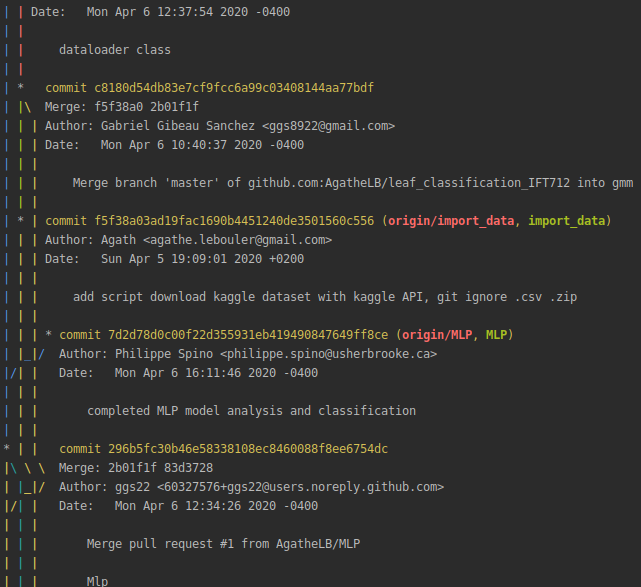
\includegraphics[width=15cm]{images/git_graph.png}
        \caption{Apperçu de l'arborescence du Git}
        \label{fig:git_graph}
    \end{figure}
    \newpage
    \section{Conclusion et pistes de recherche future}
    
    \pagebreak
    % Appendices
    %\renewcommand{\appendixname}{Annexe}
    %\begin{appendices}
    %    \input{annexea}
        
    %\end{appendices}
    \pagebreak
    
    % Bibliography
    \singlespacing
    \renewcommand{\refname}{Bibliographie}
    \bibliographystyle{IEEEtranN}
    %\bibliography{biblio}
    
\end{document}